% Options for packages loaded elsewhere
\PassOptionsToPackage{unicode}{hyperref}
\PassOptionsToPackage{hyphens}{url}
%
\documentclass[
  man]{apa6}
\usepackage{amsmath,amssymb}
\usepackage{lmodern}
\usepackage{iftex}
\ifPDFTeX
  \usepackage[T1]{fontenc}
  \usepackage[utf8]{inputenc}
  \usepackage{textcomp} % provide euro and other symbols
\else % if luatex or xetex
  \usepackage{unicode-math}
  \defaultfontfeatures{Scale=MatchLowercase}
  \defaultfontfeatures[\rmfamily]{Ligatures=TeX,Scale=1}
\fi
% Use upquote if available, for straight quotes in verbatim environments
\IfFileExists{upquote.sty}{\usepackage{upquote}}{}
\IfFileExists{microtype.sty}{% use microtype if available
  \usepackage[]{microtype}
  \UseMicrotypeSet[protrusion]{basicmath} % disable protrusion for tt fonts
}{}
\makeatletter
\@ifundefined{KOMAClassName}{% if non-KOMA class
  \IfFileExists{parskip.sty}{%
    \usepackage{parskip}
  }{% else
    \setlength{\parindent}{0pt}
    \setlength{\parskip}{6pt plus 2pt minus 1pt}}
}{% if KOMA class
  \KOMAoptions{parskip=half}}
\makeatother
\usepackage{xcolor}
\usepackage{graphicx}
\makeatletter
\def\maxwidth{\ifdim\Gin@nat@width>\linewidth\linewidth\else\Gin@nat@width\fi}
\def\maxheight{\ifdim\Gin@nat@height>\textheight\textheight\else\Gin@nat@height\fi}
\makeatother
% Scale images if necessary, so that they will not overflow the page
% margins by default, and it is still possible to overwrite the defaults
% using explicit options in \includegraphics[width, height, ...]{}
\setkeys{Gin}{width=\maxwidth,height=\maxheight,keepaspectratio}
% Set default figure placement to htbp
\makeatletter
\def\fps@figure{htbp}
\makeatother
\setlength{\emergencystretch}{3em} % prevent overfull lines
\providecommand{\tightlist}{%
  \setlength{\itemsep}{0pt}\setlength{\parskip}{0pt}}
\setcounter{secnumdepth}{-\maxdimen} % remove section numbering
% Make \paragraph and \subparagraph free-standing
\ifx\paragraph\undefined\else
  \let\oldparagraph\paragraph
  \renewcommand{\paragraph}[1]{\oldparagraph{#1}\mbox{}}
\fi
\ifx\subparagraph\undefined\else
  \let\oldsubparagraph\subparagraph
  \renewcommand{\subparagraph}[1]{\oldsubparagraph{#1}\mbox{}}
\fi
\newlength{\cslhangindent}
\setlength{\cslhangindent}{1.5em}
\newlength{\csllabelwidth}
\setlength{\csllabelwidth}{3em}
\newlength{\cslentryspacingunit} % times entry-spacing
\setlength{\cslentryspacingunit}{\parskip}
\newenvironment{CSLReferences}[2] % #1 hanging-ident, #2 entry spacing
 {% don't indent paragraphs
  \setlength{\parindent}{0pt}
  % turn on hanging indent if param 1 is 1
  \ifodd #1
  \let\oldpar\par
  \def\par{\hangindent=\cslhangindent\oldpar}
  \fi
  % set entry spacing
  \setlength{\parskip}{#2\cslentryspacingunit}
 }%
 {}
\usepackage{calc}
\newcommand{\CSLBlock}[1]{#1\hfill\break}
\newcommand{\CSLLeftMargin}[1]{\parbox[t]{\csllabelwidth}{#1}}
\newcommand{\CSLRightInline}[1]{\parbox[t]{\linewidth - \csllabelwidth}{#1}\break}
\newcommand{\CSLIndent}[1]{\hspace{\cslhangindent}#1}
\ifLuaTeX
\usepackage[bidi=basic]{babel}
\else
\usepackage[bidi=default]{babel}
\fi
\babelprovide[main,import]{english}
% get rid of language-specific shorthands (see #6817):
\let\LanguageShortHands\languageshorthands
\def\languageshorthands#1{}
% Manuscript styling
\usepackage{upgreek}
\captionsetup{font=singlespacing,justification=justified}

% Table formatting
\usepackage{longtable}
\usepackage{lscape}
% \usepackage[counterclockwise]{rotating}   % Landscape page setup for large tables
\usepackage{multirow}		% Table styling
\usepackage{tabularx}		% Control Column width
\usepackage[flushleft]{threeparttable}	% Allows for three part tables with a specified notes section
\usepackage{threeparttablex}            % Lets threeparttable work with longtable

% Create new environments so endfloat can handle them
% \newenvironment{ltable}
%   {\begin{landscape}\centering\begin{threeparttable}}
%   {\end{threeparttable}\end{landscape}}
\newenvironment{lltable}{\begin{landscape}\centering\begin{ThreePartTable}}{\end{ThreePartTable}\end{landscape}}

% Enables adjusting longtable caption width to table width
% Solution found at http://golatex.de/longtable-mit-caption-so-breit-wie-die-tabelle-t15767.html
\makeatletter
\newcommand\LastLTentrywidth{1em}
\newlength\longtablewidth
\setlength{\longtablewidth}{1in}
\newcommand{\getlongtablewidth}{\begingroup \ifcsname LT@\roman{LT@tables}\endcsname \global\longtablewidth=0pt \renewcommand{\LT@entry}[2]{\global\advance\longtablewidth by ##2\relax\gdef\LastLTentrywidth{##2}}\@nameuse{LT@\roman{LT@tables}} \fi \endgroup}

% \setlength{\parindent}{0.5in}
% \setlength{\parskip}{0pt plus 0pt minus 0pt}

% Overwrite redefinition of paragraph and subparagraph by the default LaTeX template
% See https://github.com/crsh/papaja/issues/292
\makeatletter
\renewcommand{\paragraph}{\@startsection{paragraph}{4}{\parindent}%
  {0\baselineskip \@plus 0.2ex \@minus 0.2ex}%
  {-1em}%
  {\normalfont\normalsize\bfseries\itshape\typesectitle}}

\renewcommand{\subparagraph}[1]{\@startsection{subparagraph}{5}{1em}%
  {0\baselineskip \@plus 0.2ex \@minus 0.2ex}%
  {-\z@\relax}%
  {\normalfont\normalsize\itshape\hspace{\parindent}{#1}\textit{\addperi}}{\relax}}
\makeatother

% \usepackage{etoolbox}
\makeatletter
\patchcmd{\HyOrg@maketitle}
  {\section{\normalfont\normalsize\abstractname}}
  {\section*{\normalfont\normalsize\abstractname}}
  {}{\typeout{Failed to patch abstract.}}
\patchcmd{\HyOrg@maketitle}
  {\section{\protect\normalfont{\@title}}}
  {\section*{\protect\normalfont{\@title}}}
  {}{\typeout{Failed to patch title.}}
\makeatother

\usepackage{xpatch}
\makeatletter
\xapptocmd\appendix
  {\xapptocmd\section
    {\addcontentsline{toc}{section}{\appendixname\ifoneappendix\else~\theappendix\fi\\: #1}}
    {}{\InnerPatchFailed}%
  }
{}{\PatchFailed}
\DeclareDelayedFloatFlavor{ThreePartTable}{table}
\DeclareDelayedFloatFlavor{lltable}{table}
\DeclareDelayedFloatFlavor*{longtable}{table}
\makeatletter
\renewcommand{\efloat@iwrite}[1]{\immediate\expandafter\protected@write\csname efloat@post#1\endcsname{}}
\makeatother
\usepackage{csquotes}
\ifLuaTeX
  \usepackage{selnolig}  % disable illegal ligatures
\fi
\IfFileExists{bookmark.sty}{\usepackage{bookmark}}{\usepackage{hyperref}}
\IfFileExists{xurl.sty}{\usepackage{xurl}}{} % add URL line breaks if available
\urlstyle{same} % disable monospaced font for URLs
\hypersetup{
  pdftitle={TRABAJO APLICADO ESTADÍSTICA INFERENCIAL},
  pdfauthor={Santiago Cubillos Cruz},
  pdflang={en-EN},
  hidelinks,
  pdfcreator={LaTeX via pandoc}}

\title{TRABAJO APLICADO ESTADÍSTICA INFERENCIAL}
\author{Santiago Cubillos Cruz\textsuperscript{}}
\date{}


\shorttitle{Analisis ,interpretacion y conclusiones}

\affiliation{\phantom{0}}

\note{

Universidad del Rosario

Facultad de Administración de empresas

Inferencia Estadística

Docente: Adriana Paola pachón Gutierrez

}

\begin{document}
\maketitle

\hypertarget{introducciuxf3n}{%
\section{Introducción}\label{introducciuxf3n}}

Esta muestra es resultado de la iniciativa de estudiantes de psicología
de la universidad de antioquia para conocer conceptos básicos sobre los
estudiantes que entran a la universidad basándose en la prueba de estado
presentada antes de entrar a la universidad y los resultados del primer
semestre . Se realiza una selección de 11 variables de las 22 variables
en total recogidas.Las variables escogidas se dan de manera natural en
el entendimiento ,y relación de los valores de un examen de estado y la
dedicación durante el semestre .Durante el el presente trabajo
expondremos las principales características del conjunto de datos y
pondremos en juicio algunas de las preguntas presentadas por el equipo
psicológico que tomó la muestra.

\hypertarget{planteamiento-del-problema}{%
\section{Planteamiento del Problema}\label{planteamiento-del-problema}}

¿Existe una relación intrínseca entre las notas obtenidas por los
estudiantes en las pruebas de estado y el promedio del primer semestre?

\hypertarget{objetivo-general}{%
\section{Objetivo General}\label{objetivo-general}}

-Identificar las variables que intervienen activamente en la obtención
del puntaje promedio en primer semestre

\hypertarget{objetivo-especifico}{%
\subsection{Objetivo Especifico}\label{objetivo-especifico}}

-Analizar las variables y sus relaciones para poder saber si existe una
correlación entre las notas , otras variables y el promedio como
variable respuesta . \newpage

\hypertarget{definiciuxf3n-de-variables}{%
\section{Definición de Variables}\label{definiciuxf3n-de-variables}}

\hypertarget{variables-cualitativas}{%
\subsection{Variables Cualitativas}\label{variables-cualitativas}}

Escala Nominal:

\begin{itemize}

  \item Genero :F-femenino ,M-masculino  
  \item ¿Realiza actividades extracurriculares? :Si , NO
  
\end{itemize}

Escala Ordinal:

\begin{itemize}

  \item Estrato social: "1","2","3","4","5","6"
  \item ¿Repasa los temas vistos en clase? : Nunca, Pocas Veces,Algunas Veces,Casi siempre , Siempre 
  
\end{itemize}

\hypertarget{variables-cuantitativas}{%
\subsection{Variables Cuantitativas}\label{variables-cuantitativas}}

Discreta :

\begin{itemize}

  \item Edad (en años) : mínimo 15 años  y máximo 25 años [razón]
  \item Tiempo de estudio semanal (horas) : mínimo 30 horas y máximo 55 horas [razón]
  \item ¿A cuántas tutorias asistió durante el semestre? : mínimo 1 y máximo 10 [razón]
  
\end{itemize}

Continua :

\begin{itemize}

  \item PUNTAJE MATEMÁTICAS : entre  32 y 55 [razón]
  \item PUNTAJE C. NATURALES : entre 47 y 73 [razón]
  \item PUNTAJE INGLES : entre 37 y 63 [razón]
  \item Promedio Primer Semestre : entre 3.0  y 4.9 [razón]
  
\end{itemize}

\hypertarget{anuxe1lisis-de-datos-cuantitativos}{%
\section{Análisis de datos Cuantitativos}\label{anuxe1lisis-de-datos-cuantitativos}}

Se establecerán las principales características de las variables
cuantitativas encontradas en la investigación .

\hypertarget{edad-en-auxf1os}{%
\subsection{Edad (en años)}\label{edad-en-auxf1os}}

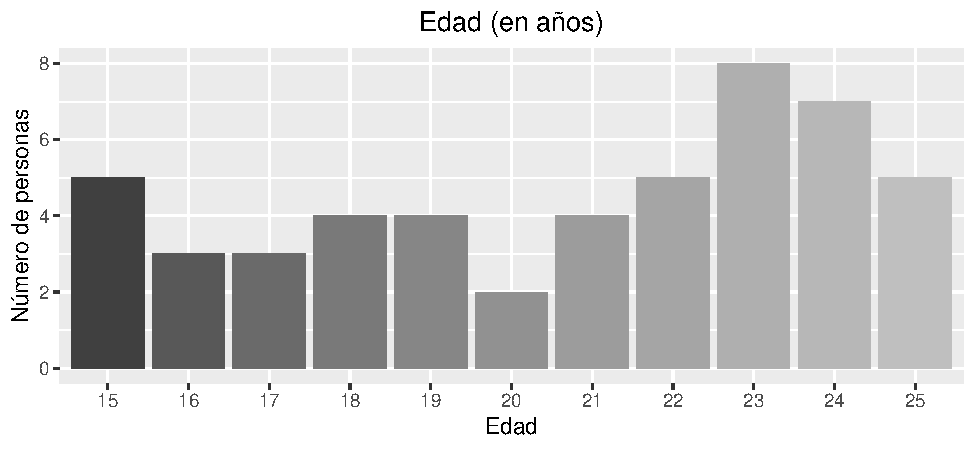
\includegraphics{Trabajo-Inferencia-estadística_files/figure-latex/edad-1.pdf}
Se observa uniformidad en la cantidad de estudiantes por cada edad
además de que al ser universitarios están entre los 15 y 25 años.
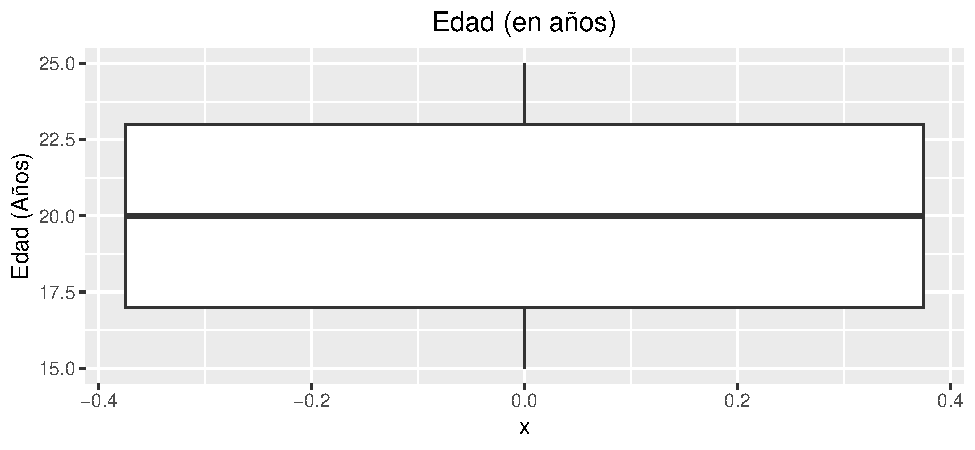
\includegraphics{Trabajo-Inferencia-estadística_files/figure-latex/edadBox-1.pdf}

la distribución de los datos parece no tener datos atípicos .

Tabla 1 : Descripción numérica para la variable Edad.

\begin{center}

\begin{tabular}{l|r}
\hline
  & Datos\\
\hline
Promedio & 20.15\\
\hline
Mediana & 20.00\\
\hline
Varianza & 10.56\\
\hline
SD & 3.25\\
\hline
CV & 16.12\\
\hline
Q1 & 17.00\\
\hline
Q2 & 20.00\\
\hline
Q3 & 23.00\\
\hline
Minimo & 15.00\\
\hline
Maximo & 25.00\\
\hline
\end{tabular}
\end{center}

CV es menor al 20\% la media será una buena medida descriptiva de la
centralidad edad de los estudiantes universitarios.

Tabla 2 : Tabla de frecuencias para la edad

\begin{center}


\begin{tabular}{r|r|r|r|r|r|r}
\hline
Lower & Upper & Main & Frequency & Percentage & CF & CPF\\
\hline
15 & 16 & 15.5 & 37 & 16.8 & 37 & 16.8\\
\hline
16 & 17 & 16.5 & 24 & 10.9 & 61 & 27.7\\
\hline
17 & 18 & 17.5 & 19 & 8.6 & 80 & 36.4\\
\hline
18 & 19 & 18.5 & 22 & 10.0 & 102 & 46.4\\
\hline
19 & 20 & 19.5 & 12 & 5.5 & 114 & 51.8\\
\hline
20 & 21 & 20.5 & 15 & 6.8 & 129 & 58.6\\
\hline
21 & 22 & 21.5 & 19 & 8.6 & 148 & 67.3\\
\hline
22 & 23 & 22.5 & 26 & 11.8 & 174 & 79.1\\
\hline
23 & 24 & 23.5 & 27 & 12.3 & 201 & 91.4\\
\hline
24 & 25 & 24.5 & 19 & 8.6 & 220 & 100.0\\
\hline
\end{tabular}
\end{center}

\hypertarget{tiempo-de-estudio-semanal-en-horas}{%
\subsection{Tiempo de estudio semanal (en horas)}\label{tiempo-de-estudio-semanal-en-horas}}

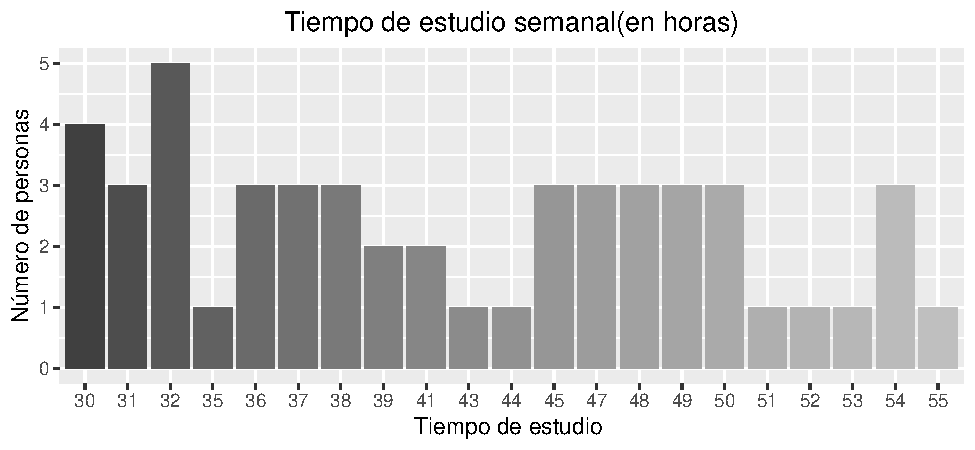
\includegraphics{Trabajo-Inferencia-estadística_files/figure-latex/tiempo-1.pdf}

Se observa uniformidad en la cantidad de tiempo dedicado al estudio por
los estudiantes .

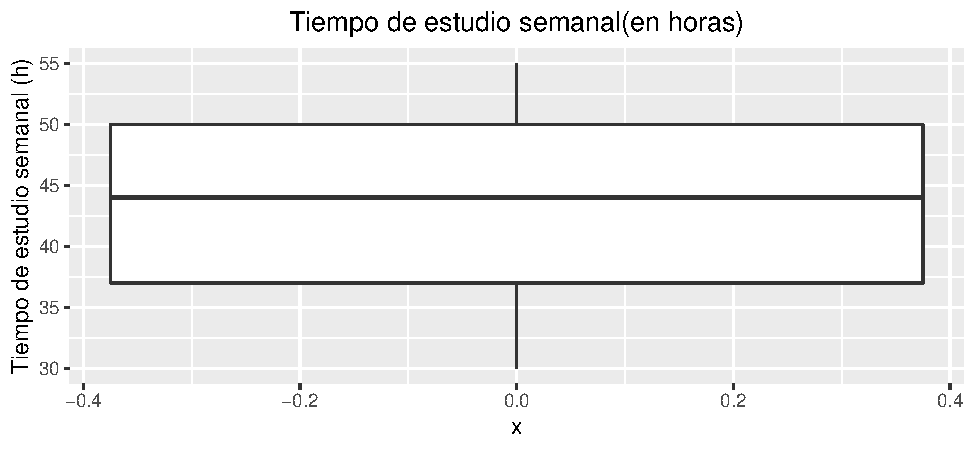
\includegraphics{Trabajo-Inferencia-estadística_files/figure-latex/tiempoBox-1.pdf}

la distribución de los datos parece no tener datos atípicos . \clearpage

Tabla 3 : Descripción numérica para la variable Tiempo de estudio
semanal.

\begin{center}

\begin{tabular}{l|r}
\hline
  & Datos\\
\hline
Promedio & 43.18\\
\hline
Mediana & 44.00\\
\hline
Varianza & 58.01\\
\hline
SD & 7.62\\
\hline
CV & 17.64\\
\hline
Q1 & 37.00\\
\hline
Q2 & 44.00\\
\hline
Q3 & 50.00\\
\hline
Minimo & 30.00\\
\hline
Maximo & 55.00\\
\hline
\end{tabular}
\end{center}

CV es menor al 20\% la media será una buena medida descriptiva de la
centralidad del tiempo de estudio semanal de los estudiantes
universitarios.

Tabla 4 : Tabla de frecuencias para el tiempo de estudio semanal (en
horas)

\begin{center}


\begin{tabular}{r|r|r|r|r|r|r}
\hline
Lower & Upper & Main & Frequency & Percentage & CF & CPF\\
\hline
30 & 35 & 32.5 & 42 & 19.1 & 42 & 19.1\\
\hline
35 & 40 & 37.5 & 42 & 19.1 & 84 & 38.2\\
\hline
40 & 45 & 42.5 & 38 & 17.3 & 122 & 55.5\\
\hline
45 & 50 & 47.5 & 50 & 22.7 & 172 & 78.2\\
\hline
50 & 55 & 52.5 & 48 & 21.8 & 220 & 100.0\\
\hline
\end{tabular}
\end{center}

\hypertarget{nuxfamero-de-tutorias}{%
\subsection{Número de tutorias}\label{nuxfamero-de-tutorias}}

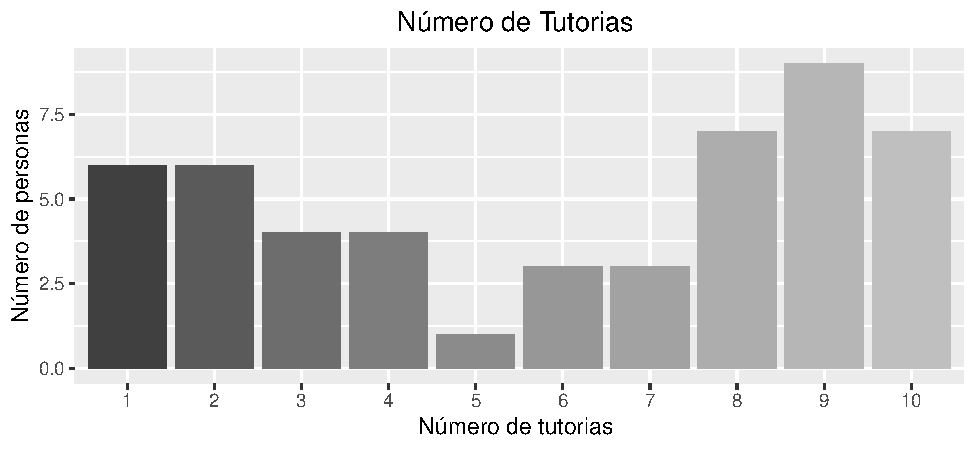
\includegraphics{Trabajo-Inferencia-estadística_files/figure-latex/tutorias-1.pdf}

Se observa uniformidad en la cantidad de tiempo dedicado al estudio por
los estudiantes .

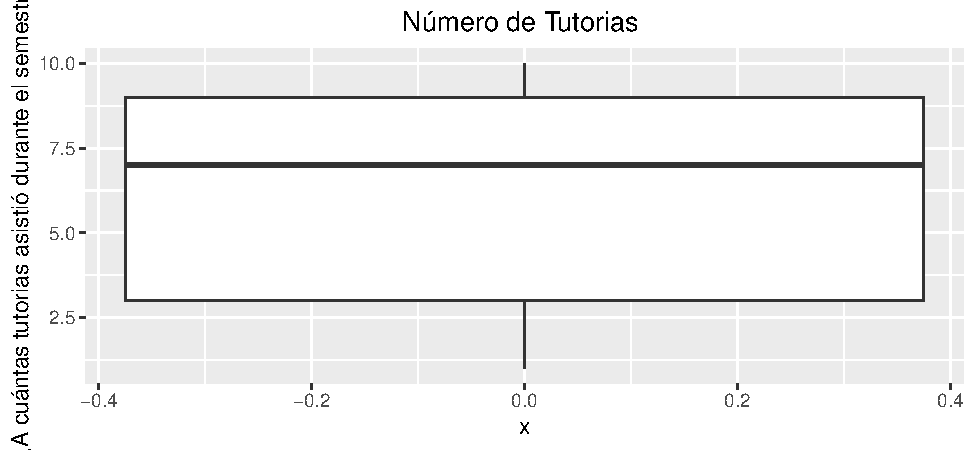
\includegraphics{Trabajo-Inferencia-estadística_files/figure-latex/tutoriasBox-1.pdf}

la distribución de los datos parece no tener datos atípicos . \clearpage

Tabla 5 : Descripción numérica para la variable del número de horas de
estudio

\begin{center}

\begin{tabular}{l|r}
\hline
  & Datos\\
\hline
Promedio & 5.71\\
\hline
Mediana & 6.00\\
\hline
Varianza & 9.48\\
\hline
SD & 3.08\\
\hline
CV & 53.92\\
\hline
Q1 & 3.00\\
\hline
Q2 & 6.00\\
\hline
Q3 & 9.00\\
\hline
Minimo & 1.00\\
\hline
Maximo & 10.00\\
\hline
\end{tabular}
\end{center}

CV es mayor al 20\% la media será tan buena medida descriptiva de la
centralidad del número de tutorias que toman los estudiantes
universitarios.

Tabla 6 : Tabla de frecuencias para el número de horas de estudio

\begin{center}


\begin{tabular}{r|r|r|r|r|r|r}
\hline
Lower & Upper & Main & Frequency & Percentage & CF & CPF\\
\hline
1 & 2 & 1.5 & 46 & 20.9 & 46 & 20.9\\
\hline
2 & 3 & 2.5 & 23 & 10.5 & 69 & 31.4\\
\hline
3 & 4 & 3.5 & 21 & 9.5 & 90 & 40.9\\
\hline
4 & 5 & 4.5 & 13 & 5.9 & 103 & 46.8\\
\hline
5 & 6 & 5.5 & 16 & 7.3 & 119 & 54.1\\
\hline
6 & 7 & 6.5 & 21 & 9.5 & 140 & 63.6\\
\hline
7 & 8 & 7.5 & 24 & 10.9 & 164 & 74.5\\
\hline
8 & 9 & 8.5 & 25 & 11.4 & 189 & 85.9\\
\hline
9 & 10 & 9.5 & 31 & 14.1 & 220 & 100.0\\
\hline
\end{tabular}
\end{center}

\hypertarget{puntaje-en-matemuxe1ticas}{%
\subsection{Puntaje en Matemáticas}\label{puntaje-en-matemuxe1ticas}}

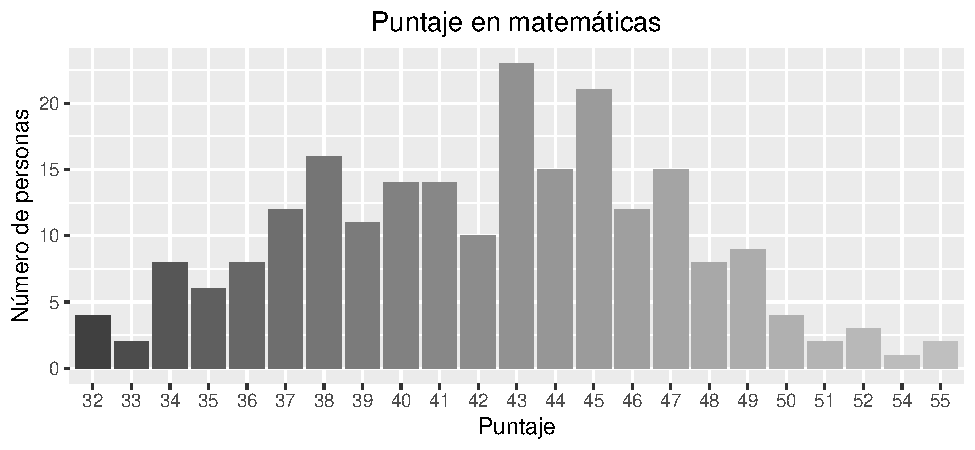
\includegraphics{Trabajo-Inferencia-estadística_files/figure-latex/math-1.pdf}

Es observable que el puntaje tiende a acercarse a la media haciendo las
colas menos pesadas .

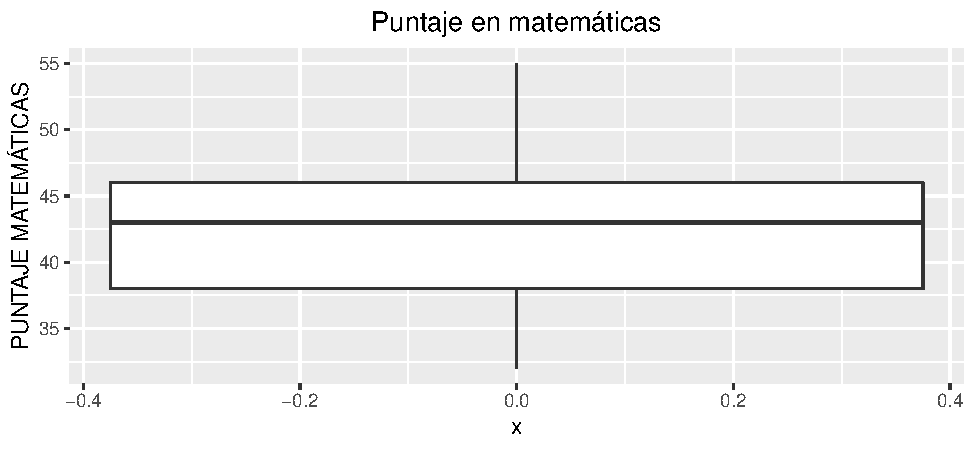
\includegraphics{Trabajo-Inferencia-estadística_files/figure-latex/mathBox-1.pdf}

la distribución de los datos parece no tener datos atípicos . \clearpage
Tabla 7 : Descripción numérica para el puntaje en matemáticas

\begin{center}

\begin{tabular}{l|r}
\hline
  & Datos\\
\hline
Promedio & 42.26\\
\hline
Mediana & 43.00\\
\hline
Varianza & 23.44\\
\hline
SD & 4.84\\
\hline
CV & 11.46\\
\hline
Q1 & 38.00\\
\hline
Q2 & 43.00\\
\hline
Q3 & 46.00\\
\hline
Minimo & 32.00\\
\hline
Maximo & 55.00\\
\hline
\end{tabular}
\end{center}

CV es menor al 20\% la media será una buena medida descriptiva de la
centralidad del puntaje en matemáticas de los estudiantes
universitarios.

Tabla 8 : Tabla de frecuencias para el puntaje en matemáticas

\begin{center}


\begin{tabular}{r|r|r|r|r|r|r}
\hline
Lower & Upper & Main & Frequency & Percentage & CF & CPF\\
\hline
30 & 35 & 32.5 & 20 & 9.1 & 20 & 9.1\\
\hline
35 & 40 & 37.5 & 61 & 27.7 & 81 & 36.8\\
\hline
40 & 45 & 42.5 & 83 & 37.7 & 164 & 74.5\\
\hline
45 & 50 & 47.5 & 48 & 21.8 & 212 & 96.4\\
\hline
50 & 55 & 52.5 & 8 & 3.6 & 220 & 100.0\\
\hline
\end{tabular}
\end{center}

\hypertarget{puntaje-en-ciencias-naturales}{%
\subsection{Puntaje en Ciencias Naturales}\label{puntaje-en-ciencias-naturales}}

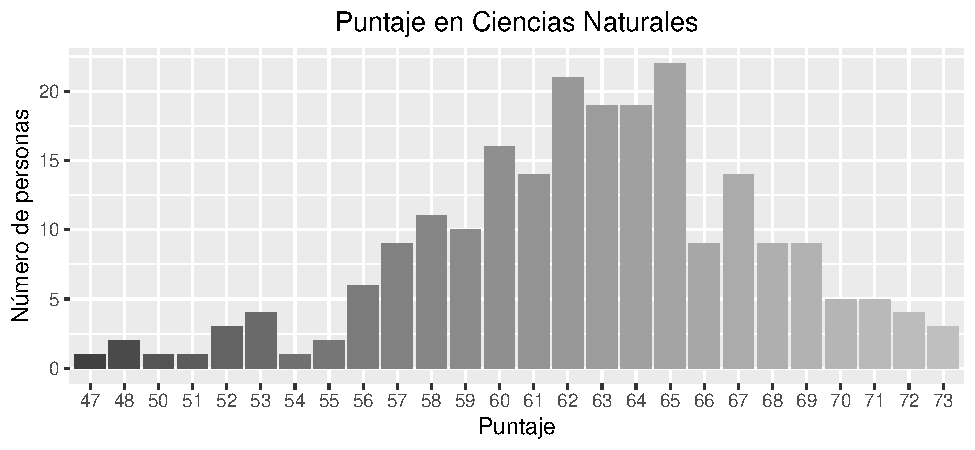
\includegraphics{Trabajo-Inferencia-estadística_files/figure-latex/nat-1.pdf}

Es observable que el puntaje tiende a acercarse a la media haciendo las
colas menos pesadas .

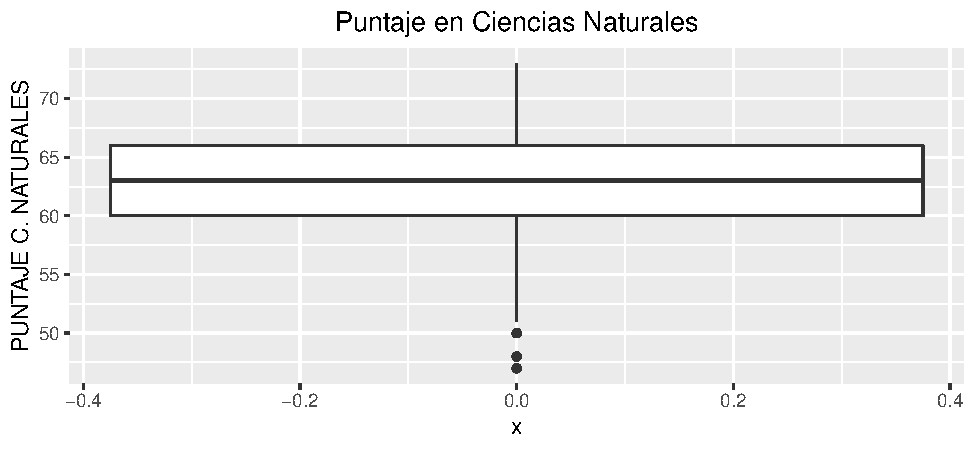
\includegraphics{Trabajo-Inferencia-estadística_files/figure-latex/nathBox-1.pdf}

la distribución parece ser apuntada a la media y posee datos atípicos .
\clearpage Tabla 9 : Descripción numérica para el puntaje en ciencias
naturales

\begin{center}

\begin{tabular}{l|r}
\hline
  & Datos\\
\hline
Promedio & 62.68\\
\hline
Mediana & 63.00\\
\hline
Varianza & 24.62\\
\hline
SD & 4.96\\
\hline
CV & 7.92\\
\hline
Q1 & 60.00\\
\hline
Q2 & 63.00\\
\hline
Q3 & 66.00\\
\hline
Minimo & 47.00\\
\hline
Maximo & 73.00\\
\hline
\end{tabular}
\end{center}

CV es menor al 20\% la media será una buena medida descriptiva de la
centralidad del puntaje en ciencias naturales de los estudiantes
universitarios cabe notar la poca variación de los datos frente a la
media aunque existen valores atípicos.

Tabla 10 : Tabla de frecuencias para el puntaje en ciencias naturales

\begin{center}


\begin{tabular}{r|r|r|r|r|r|r}
\hline
Lower & Upper & Main & Frequency & Percentage & CF & CPF\\
\hline
45 & 50 & 47.5 & 4 & 1.8 & 4 & 1.8\\
\hline
50 & 55 & 52.5 & 11 & 5.0 & 15 & 6.8\\
\hline
55 & 60 & 57.5 & 52 & 23.6 & 67 & 30.5\\
\hline
60 & 65 & 62.5 & 95 & 43.2 & 162 & 73.6\\
\hline
65 & 70 & 67.5 & 46 & 20.9 & 208 & 94.5\\
\hline
70 & 75 & 72.5 & 12 & 5.5 & 220 & 100.0\\
\hline
\end{tabular}
\end{center}

\hypertarget{puntaje-en-ingluxe9s}{%
\subsection{Puntaje en Inglés}\label{puntaje-en-ingluxe9s}}

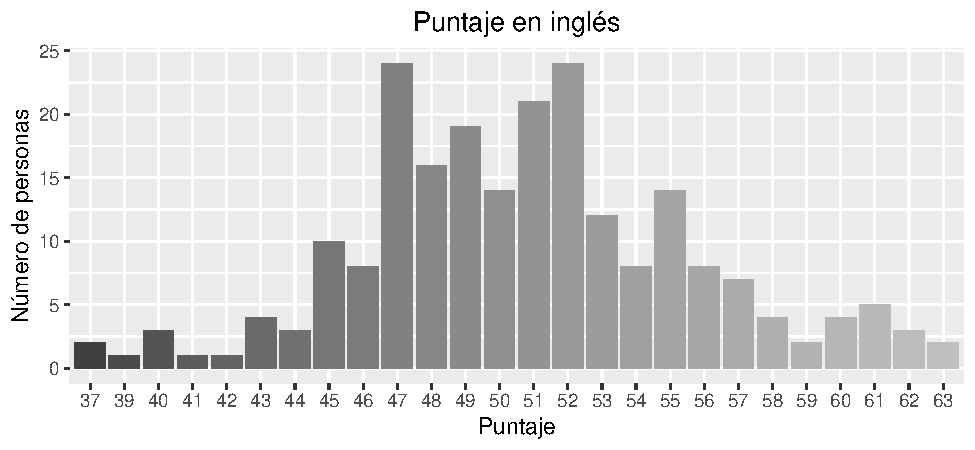
\includegraphics{Trabajo-Inferencia-estadística_files/figure-latex/ing-1.pdf}

Es observable que e puntaje tiende a acercarse a la media haciendo las
colas menos pesadas .

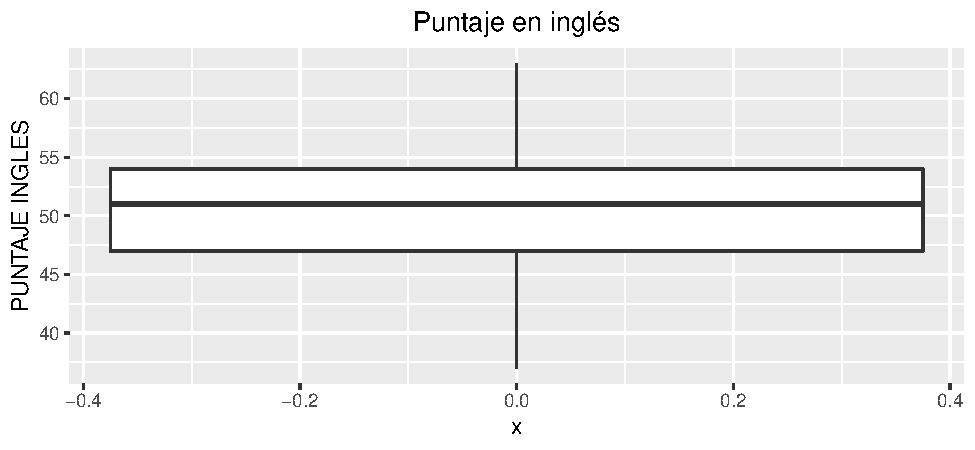
\includegraphics{Trabajo-Inferencia-estadística_files/figure-latex/inghBox-1.pdf}

la distribución parece ser apuntada a la media y no posee datos atípicos.
. \clearpage Tabla 11 : Descripción numérica para el puntaje en inglés

\begin{center}

\begin{tabular}{l|r}
\hline
  & Datos\\
\hline
Promedio & 50.80\\
\hline
Mediana & 51.00\\
\hline
Varianza & 24.07\\
\hline
SD & 4.91\\
\hline
CV & 9.66\\
\hline
Q1 & 47.00\\
\hline
Q2 & 51.00\\
\hline
Q3 & 54.00\\
\hline
Minimo & 37.00\\
\hline
Maximo & 63.00\\
\hline
\end{tabular}
\end{center}

CV es menor al 20\% la media será una buena medida descriptiva del
puntaje en inglés de los estudiantes universitarios cabe notar la poca
variación de los datos frente a la media .

Tabla 12 : Tabla de frecuencias para el puntaje en inglés

\begin{center}


\begin{tabular}{r|r|r|r|r|r|r}
\hline
Lower & Upper & Main & Frequency & Percentage & CF & CPF\\
\hline
35 & 40 & 37.5 & 6 & 2.7 & 6 & 2.7\\
\hline
40 & 45 & 42.5 & 19 & 8.6 & 25 & 11.4\\
\hline
45 & 50 & 47.5 & 81 & 36.8 & 106 & 48.2\\
\hline
50 & 55 & 52.5 & 79 & 35.9 & 185 & 84.1\\
\hline
55 & 60 & 57.5 & 25 & 11.4 & 210 & 95.5\\
\hline
60 & 65 & 62.5 & 10 & 4.5 & 220 & 100.0\\
\hline
\end{tabular}
\end{center}

\hypertarget{promedio-del-primer-semestre}{%
\subsection{Promedio del Primer Semestre}\label{promedio-del-primer-semestre}}

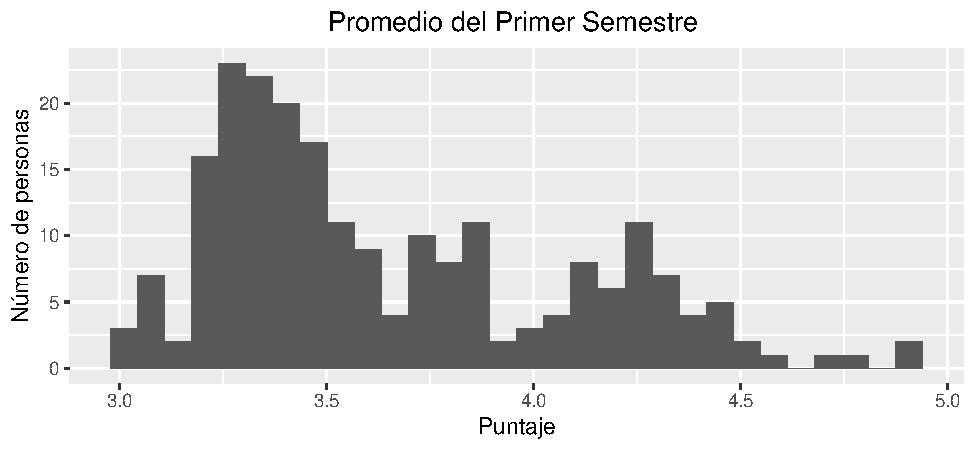
\includegraphics{Trabajo-Inferencia-estadística_files/figure-latex/pro-1.pdf}

Es observable que el puntaje tiende a acercarse a la media haciendo las
colas menos pesadas .

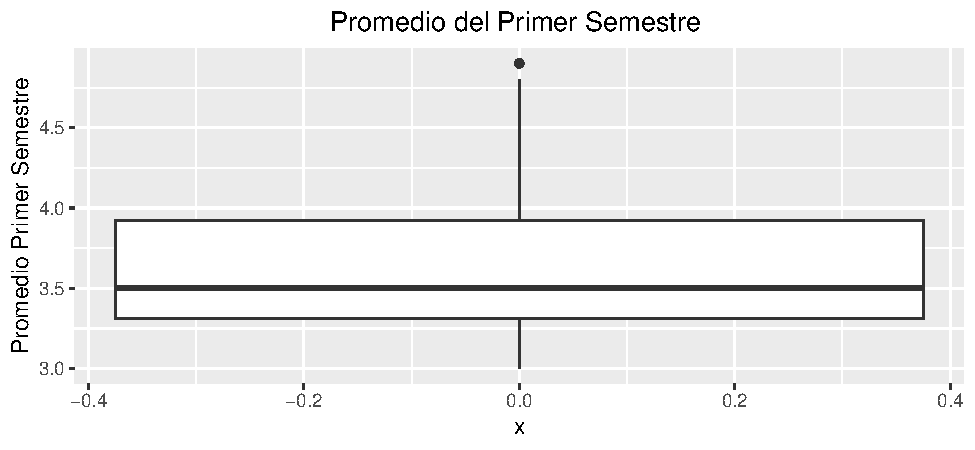
\includegraphics{Trabajo-Inferencia-estadística_files/figure-latex/proBox-1.pdf}

la distribución parece ser apuntada a dos puntos de acumulación y posee
algunos valores atípicos. \clearpage Tabla 13 : Descripción numérica
para el promedio del primer semestre

\begin{center}

\begin{tabular}{l|r}
\hline
  & Datos\\
\hline
Promedio & 3.66\\
\hline
Mediana & 3.50\\
\hline
Varianza & 0.19\\
\hline
SD & 0.43\\
\hline
CV & 11.78\\
\hline
Q1 & 3.31\\
\hline
Q2 & 3.50\\
\hline
Q3 & 3.92\\
\hline
Minimo & 3.00\\
\hline
Maximo & 4.90\\
\hline
\end{tabular}
\end{center}

CV es menor al 20\% la media será una buena medida descriptiva del
promedio del primer semestre de los estudiantes universitarios cabe
notar la poca variación de los datos frente a la media .

Tabla 14 : Tabla de frecuencias para el promedio del primer semestre

\begin{center}


\begin{tabular}{r|r|r|r|r|r|r}
\hline
Lower & Upper & Main & Frequency & Percentage & CF & CPF\\
\hline
3.0 & 3.5 & 3.25 & 110 & 50.0 & 110 & 50.0\\
\hline
3.5 & 4.0 & 3.75 & 55 & 25.0 & 165 & 75.0\\
\hline
4.0 & 4.5 & 4.25 & 50 & 22.7 & 215 & 97.7\\
\hline
4.5 & 5.0 & 4.75 & 5 & 2.3 & 220 & 100.0\\
\hline
\end{tabular}
\end{center}

\clearpage

\hypertarget{intervalos-de-confianza}{%
\section{Intervalos De Confianza}\label{intervalos-de-confianza}}

\hypertarget{intervalos-para-la-media}{%
\subsection{Intervalos para la media}\label{intervalos-para-la-media}}

Edad (en años) : mínimo 15 años y máximo 25 años {[}razón{]}

\begin{verbatim}
## [1] 19.72274 20.58635
## attr(,"conf.level")
## [1] 0.95
\end{verbatim}

Interpretación: al extraer 100 veces la muestra cada una con 221
individuos , se espera que aproximadamente 95 de estas muestras tendrán
una media de edad entre los 19.7 años y 20.6 años.

Tiempo de estudio semanal (horas) : mínimo 30 horas y máximo 55 horas
{[}razón{]}

\begin{verbatim}
## [1] 42.16524 44.18930
## attr(,"conf.level")
## [1] 0.95
\end{verbatim}

Interpretación: al extraer 100 veces la muestra cada una con 221
individuos , se espera que aproximadamente 95 de estas muestras tendrán
una media para el tiempo de estudio semanal entre 42 y 44 horas cabe
aclarar que la distribución del tiempo semanal resulto aproximadamente
uniforme .
\newpage
¿A cuántas tutorias asistió durante el semestre? : mínimo 1 y máximo 10
{[}razón{]}

\begin{verbatim}
## [1] 5.300047 6.118135
## attr(,"conf.level")
## [1] 0.95
\end{verbatim}

Interpretación: al extraer 100 veces la muestra cada una con 221
individuos , se espera que aproximadamente 95 de estas muestras tendrán
una media para el número de tutorias semanales entre 5 horas y 6 horas
de tutorias

PUNTAJE MATEMÁTICAS : entre 32 y 55 {[}razón{]}

\begin{verbatim}
## [1] 41.61572 42.90246
## attr(,"conf.level")
## [1] 0.95
\end{verbatim}

Interpretación: al extraer 100 veces la muestra cada una con 221
individuos , se espera que aproximadamente 95 de estas muestras tendrán
una nota media entre 41.61 y 42.25

PUNTAJE C. NATURALES : entre 47 y 73 {[}razón{]}

\begin{verbatim}
## [1] 62.01795 63.33660
## attr(,"conf.level")
## [1] 0.95
\end{verbatim}

Interpretación: al extraer 100 veces la muestra cada una con 221
individuos , se espera que aproximadamente 95 de estas muestras tendrán
una nota media entre 62 y 63.33
\newpage
PUNTAJE INGLES : entre 37 y 63 {[}razón{]}

\begin{verbatim}
## [1] 50.14811 51.45189
## attr(,"conf.level")
## [1] 0.95
\end{verbatim}

Interpretación: al extraer 100 veces la muestra cada una con 221
individuos , se espera que aproximadamente 95 de estas muestras tendrán
una nota media entre 50.14 y 51.45

Promedio Primer Semestre : entre 3.0 y 4.9 {[}razón{]}

\begin{verbatim}
## [1] 3.598850 3.713283
## attr(,"conf.level")
## [1] 0.95
\end{verbatim}

Interpretación: al extraer 100 veces la muestra cada una con 221
individuos , se espera que aproximadamente 95 de estas muestras tendrán
una nota media del promedio general del primer semestre entre 3.59 y
3.71
\newpage

\hypertarget{intervalo-de-confianza-para-la-proporciuxf3n}{%
\subsection{Intervalo de confianza para la proporción}\label{intervalo-de-confianza-para-la-proporciuxf3n}}

Se desea obtener un intervalo de confianza para la proporción de los estudiantes que
tienen mas de 4 , recordemos que :
\[
IC_{1-\alpha}(p)=[\hat p \mp z_{\frac{\alpha}{2}}\sqrt{\frac{\hat p (1-\hat p)}{n}}]
\]
entonces el intervalo será :

\[
IC_{1-\alpha}(p)=[0.25\mp 1.96 *\sqrt{\frac{0.25*0.75}{220}}]=(0.1927803,0.3072197)
\]

Interpretación:al extraer 100 veces la muestra cada una con 221
individuos , se espera que aproximadamente 95 de estas muestras tendrán
una proporción para las personas que obtiene una nota por encima entre 19.28\% y
30.72\%

\hypertarget{intervalo-de-confianza-para-la-varianza}{%
\subsection{Intervalo de confianza para la varianza}\label{intervalo-de-confianza-para-la-varianza}}

estimamos un intervalo de confianza para la varianza de la nota promedio .

\begin{verbatim}
## [1] 0.1550600 0.2257113
## attr(,"conf.level")
## [1] 0.95
\end{verbatim}

Interpretación:al extraer 100 veces la muestra cada una con 221
individuos , se espera que aproximadamente 95 de estas muestras tendrán
varianza entre 0.155 y 0.2257
\newpage

\hypertarget{pruebas-de-bondad-de-ajuste-chi-cuadrado}{%
\section{Pruebas de Bondad de Ajuste (Chi-cuadrado)}\label{pruebas-de-bondad-de-ajuste-chi-cuadrado}}

Para la prueba de independencia Chi-cuadrado se considerada la hipótesis
nula:

\[
\left\{
\begin{array}{ll}
H_{0}: &  \text{las variables son independendientes}\\
H_{1}: & \text{las variables son dependientes}
\end{array}
\right.
\]

\hypertarget{guxe9nero-estrato-social}{%
\subsection{Género-Estrato Social}\label{guxe9nero-estrato-social}}

Se observa la relación entre el género y el estrato social

\begin{center}


\begin{tabular}{l|r|r|r|r|r|r}
\hline
  & 1 & 2 & 3 & 4 & 5 & 6\\
\hline
F & 23 & 21 & 17 & 19 & 16 & 15\\
\hline
M & 18 & 20 & 18 & 17 & 21 & 15\\
\hline
\end{tabular}


    Pearson's Chi-squared test

data:  generoEstrato
X-squared = 1.4314, df = 5, p-value = 0.9208
\end{center}

la prueba chi-cuadrado nos da un p-valor de 0.9208 , para un nivel de
significancia del \(\alpha =0.05\) no hay evidencia estadística para
rechazar \(H_o\) , es decir el género y el estrato social son
independientes

\hypertarget{actividades-extracurriculares---repaso-de-temas}{%
\subsection{Actividades extracurriculares - Repaso de temas}\label{actividades-extracurriculares---repaso-de-temas}}

Se observa la relación entre el realizar actividades extracurriculares y
la pregunta ``¿repasa usted los temas vistos en clase?''

\begin{center}


\begin{tabular}{l|r|r}
\hline
  & NO & SI\\
\hline
Algunas veces & 32 & 30\\
\hline
Casi siempre & 23 & 33\\
\hline
Nunca & 18 & 20\\
\hline
Pocas veces & 5 & 18\\
\hline
Siempre & 19 & 22\\
\hline
\end{tabular}


    Pearson's Chi-squared test

data:  extraRepaso
X-squared = 6.5415, df = 4, p-value = 0.1622
\end{center}

la prueba chi-cuadrado nos da un p-valor de 0.1622 , para un nivel de
significancia del \(\alpha =0.05\) no hay evidencia estadística para
rechazar \(H_o\) , es decir el realizar actividades extracurriculares y la
pregunta ``¿repasa usted los temas vistos en clase?'' son independientes

\hypertarget{estrato-social---actividades-extracurriculares}{%
\subsection{Estrato Social - actividades extracurriculares}\label{estrato-social---actividades-extracurriculares}}

Se observa la relación entre el estrato social y el realizar actividades
extracurriculares

\begin{center}


\begin{tabular}{l|r|r|r|r|r|r}
\hline
  & 1 & 2 & 3 & 4 & 5 & 6\\
\hline
NO & 19 & 19 & 16 & 17 & 13 & 13\\
\hline
SI & 22 & 22 & 19 & 19 & 24 & 17\\
\hline
\end{tabular}


    Pearson's Chi-squared test

data:  estratoExtra
X-squared = 1.5599, df = 5, p-value = 0.9061
\end{center}

la prueba chi-cuadrado nos da un p-valor de 0.9064 , para un nivel de
significancia del \(\alpha =0.05\) no hay evidencia estadística para
rechazar \(H_o\) , es decir el estrato social y el realizar actividades
extracurriculares son independientes.

\clearpage

\hypertarget{pruebas-de-normalidad}{%
\section{Pruebas de Normalidad}\label{pruebas-de-normalidad}}

Para la prueba de normalidad se considerada la hipótesis nula:

\[
\left\{
\begin{array}{ll}
H_{0}: &  \text{La variable tiene distribución Normal}\\
H_{1}: & \text{las variables no tiene distribución normal}
\end{array}
\right.
\]
puesto que la muestra es de 220 datos se usará el test mas potente
que es el test de kolmogorov-smirnof en su variante el test de Lilie
efors

\hypertarget{prueba-para-la-edad}{%
\subsection{Prueba para la edad}\label{prueba-para-la-edad}}

\begin{center}


    Lilliefors (Kolmogorov-Smirnov) normality test

data:  Edad (Años)
D = 0.13665, p-value = 9.794e-11
\end{center}

Existe evidencia para rechazar \(H_0\) , con un nivel de significancia de
\(\alpha=0.05\) hay evidencia estadística para apoyar que la variable Edad
no se distribuye de maneral normal .

\hypertarget{prueba-para-tiempo-de-estudio-semanal}{%
\subsection{Prueba para Tiempo de estudio semanal}\label{prueba-para-tiempo-de-estudio-semanal}}

\begin{center}


    Lilliefors (Kolmogorov-Smirnov) normality test

data:  Tiempo de estudio semanal (h)
D = 0.10943, p-value = 1.009e-06
\end{center}

Existe evidencia para rechazar \(H_0\) , con un nivel de significancia de
\(\alpha=0.05\) hay evidencia estadística para apoyar que la variable
Tiempo de estudio semanal no se distribuye de manera normal .

\clearpage

\hypertarget{prueba-para-el-nuxfamero-de-tutorias}{%
\subsection{Prueba para el número de tutorias}\label{prueba-para-el-nuxfamero-de-tutorias}}

\begin{center}


    Lilliefors (Kolmogorov-Smirnov) normality test

data:  ¿A cuántas tutorias asistió durante el semestre?
D = 0.13525, p-value = 1.665e-10
\end{center}

Existe evidencia para rechazar \(H_0\) , con un nivel de significancia de
\(\alpha=0.05\) hay evidencia estadística para apoyar que la variable
número de tutorias no se distribuye de manera normal .

\hypertarget{prueba-para-el-puntaje-en-matemuxe1ticas}{%
\subsection{Prueba para el Puntaje en matemáticas}\label{prueba-para-el-puntaje-en-matemuxe1ticas}}

\begin{center}

    Lilliefors (Kolmogorov-Smirnov) normality test

data:  PUNTAJE MATEMÁTICAS
D = 0.083536, p-value = 0.0007722


    Shapiro-Wilk normality test

data:  PUNTAJE MATEMÁTICAS
W = 0.9874, p-value = 0.04939
\end{center}

Existe evidencia para rechazar \(H_0\) , con un nivel de significancia de
\(\alpha=0.05\) hay evidencia estadística para apoyar que la variable
Puntaje en matemáticas no se distribuye de manera normal .

\hypertarget{prueba-para-el-puntaje-en-ingluxe9s}{%
\subsection{Prueba para el Puntaje en Inglés}\label{prueba-para-el-puntaje-en-ingluxe9s}}

\begin{center}

    Lilliefors (Kolmogorov-Smirnov) normality test

data:  PUNTAJE INGLES
D = 0.089748, p-value = 0.0001899


    Shapiro-Wilk normality test

data:  PUNTAJE INGLES
W = 0.9844, p-value = 0.016
\end{center}

Existe evidencia para rechazar \(H_0\) , con un nivel de significancia de
\(\alpha=0.05\) hay evidencia estadística para apoyar que la variable
Puntaje en Inglés no se distribuye de manera normal .

\hypertarget{prueba-para-el-puntaje-en-ciencias-naturales}{%
\subsection{Prueba para el Puntaje en Ciencias Naturales}\label{prueba-para-el-puntaje-en-ciencias-naturales}}

\begin{center}

    Lilliefors (Kolmogorov-Smirnov) normality test

data:  PUNTAJE C. NATURALES
D = 0.077534, p-value = 0.00267


    Shapiro-Wilk normality test

data:  PUNTAJE C. NATURALES
W = 0.98188, p-value = 0.006352
\end{center}

Existe evidencia para rechazar \(H_0\) , con un nivel de significancia de
\(\alpha=0.05\) hay evidencia estadística para apoyar que la variable
Puntaje en Ciencias Naturales no se distribuye de manera normal .

\hypertarget{prueba-para-el-promedio-en-el-primer-semestre}{%
\subsection{Prueba para el Promedio en el Primer Semestre}\label{prueba-para-el-promedio-en-el-primer-semestre}}

\begin{center}


    Lilliefors (Kolmogorov-Smirnov) normality test

data:  Promedio Primer Semestre
D = 0.15422, p-value = 7.375e-14
\end{center}

Existe evidencia para rechazar \(H_0\) , con un nivel de significancia de
\(\alpha=0.05\) hay evidencia estadística para apoyar que la variable
Promedio en el primer semestre no se distribuye de manera normal.

\clearpage

\hypertarget{planteamiento-de-hipuxf3tesis}{%
\section{Planteamiento de hipótesis}\label{planteamiento-de-hipuxf3tesis}}

\hypertarget{hipuxf3tesis-estaduxedstica-para-la-media}{%
\subsection{Hipótesis estadística para la media:}\label{hipuxf3tesis-estaduxedstica-para-la-media}}

El personal de estudios psicologicos desea saber si el promedio en
matemáticas para los chicos de primer semestre es capaz de superar el
humbral general que es de 42 puntos.

realizaremos la prueba de hipótesis para una media para la variable
puntuación en matemáticas :

\[
\left\{
\begin{array}{ll}
H_{0}: &  \mu\leq 42\\
H_{1}: & \mu> 42
\end{array}
\right.
\] los datos obtenidos son los siguientes:

\(n=220, \bar{X}=42.26 ,S_x=4.84\) para el estadístico de prueba se tendrá
que :

\[T= \frac{\overline{X}-\mu_{0}}{ \frac{S_X}{\sqrt{n}} }\]

\begin{verbatim}
## 
##  One Sample t-test
## 
## data:  PUNTAJE MATEMÁTICAS
## t = 0.79368, df = 219, p-value = 0.2141
## alternative hypothesis: true mean is greater than 42
## 95 percent confidence interval:
##  41.71986      Inf
## sample estimates:
## mean of x 
##  42.25909
\end{verbatim}

La prueba nos arroja un valor p de 0.2141 , con una significancia de
\(\alpha=0.05\) no se reachaza \(H_0\) es decir el valor de la media
poblacional de la puntuación en matemáticas no supera el humbral.

\hypertarget{hipuxf3tesis-estaduxedstica-para-la-proporciuxf3n}{%
\subsection{Hipótesis estadística para la proporción :}\label{hipuxf3tesis-estaduxedstica-para-la-proporciuxf3n}}

el equipo psicologico de la universidad sugiere que tan solo el 25\% de
los estudiantes poseen una nota superior a 4.0

planteamos la hipótesis :

\[
\left\{
\begin{array}{ll}
H_{0}: &  p\leq 0.25\\
H_{1}: &  p> 0.25
\end{array}
\right.
\] donde \(p\) es la proporción de estudiantes que tiene 4 o mas en el
semestre .

puesto que \(np>5\) , \(nq>5\) y \(n>30\) es posible realizar la aproximación
de la binomial a la normal .

la proporción muestral es de \(\hat{p}=0.253\) y \(n=220\) entonces usando
el estadsítico de prueba\\
\[Z*= \frac{\overline{p} - p}{\sqrt{\frac{p(1-p)}{n}}}=0.10276\]
hallamos el valor p:

\[ p-val=P(Z\geq Z*)=P(Z\geq 0.10276)=0.4492328\] para un p-valor menor
o cercano no existe evidencia para rechazar \(H_0\)s , con una
significancia del \(\alpha=0.05\) es decir el valor de la proporción es
igual o menor a 0.25.

\clearpage

\hypertarget{hipuxf3tesis-estaduxedstica-para-la-diferencia-de-medias}{%
\subsection{Hipótesis estadística para la diferencia de medias :}\label{hipuxf3tesis-estaduxedstica-para-la-diferencia-de-medias}}

el equipo en psicologia desea saber si hay un diferencia significativa
entre el promedio de primer semestre de las personas que si realizaron
actividades curriculares y las que no .

planteamos la prueba de hipótesis :

\[
\left\{
\begin{array}{ll}
H_{0}: &  \mu_{si}-\mu_{no}= 0\\
H_{1}: &   \mu_{si}-\mu_{no}\neq 0
\end{array}
\right.
\]

primero realizamos el test para comparar varianzas :

\begin{verbatim}
## 
##  F test to compare two variances
## 
## data:  mSi$`Promedio Primer Semestre`  and  mNO$`Promedio Primer Semestre`
## F = 1.0857, num df = 122, denom df = 96, p-value = 0.6768
## alternative hypothesis: true ratio of variances is not equal to 1
## 95 percent confidence interval:
##  0.739107 1.581031
## sample estimates:
## ratio of variances 
##           1.085721
\end{verbatim}

con un pvalor de 0.6768 no se rechaza \(H_0\) , es decir las varianzas son
iguales .

\clearpage

Realizamos el test de muestras no pareadas y varianzas iguales :

\begin{verbatim}
## 
##  Two Sample t-test
## 
## data:  mSi$`Promedio Primer Semestre` and mNO$`Promedio Primer Semestre`
## t = -0.049351, df = 218, p-value = 0.9607
## alternative hypothesis: true difference in means is not equal to 0
## 95 percent confidence interval:
##  -0.1183993  0.1126148
## sample estimates:
## mean of x mean of y 
##  3.654791  3.657683
\end{verbatim}

Existe evidencia estadística para no rechazar \(H_0\) , pues el p-valor es
ded 0.8125 es demasiado alto para el valor de \(\alpha=0.05\) entonces no
hay diferencia significativa entre las medias de las personas que
realizan actividades extracurriculares .

\newpage

\hypertarget{regresiuxf3n-lineal-simple-y-muxfaltiple}{%
\section{Regresión Lineal Simple y Múltiple}\label{regresiuxf3n-lineal-simple-y-muxfaltiple}}

\hypertarget{anuxe1lisis-de-correlaciuxf3n}{%
\subsection{Análisis de Correlación}\label{anuxe1lisis-de-correlaciuxf3n}}

Es deseable observar un diagrama de correlaciones para ver la posibles
relaciones entre las varaibles y así mismo tener en cuenta las posibles
predicciones.

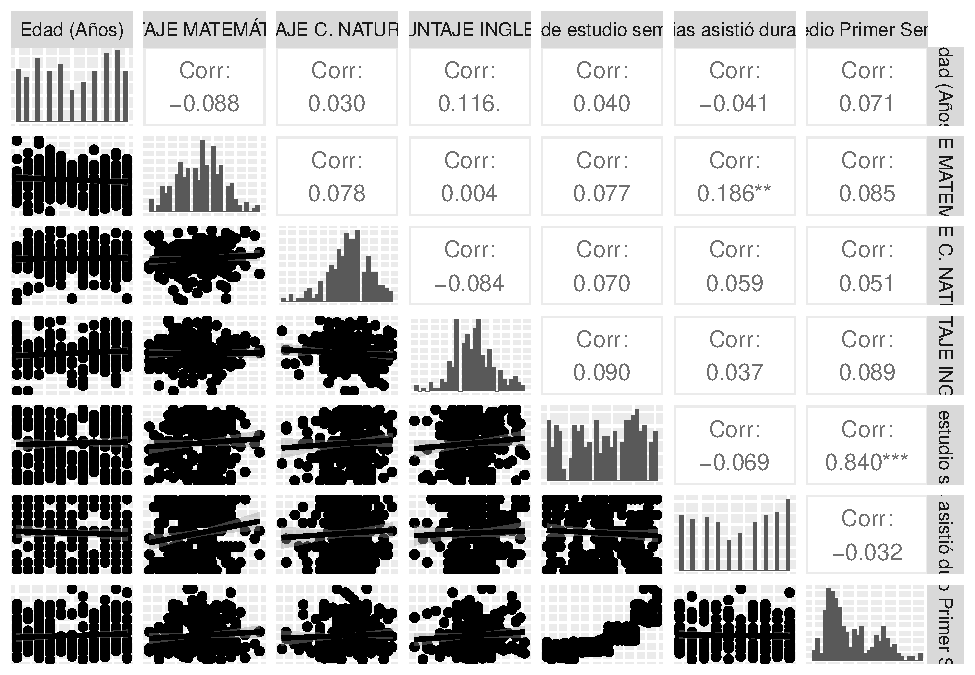
\includegraphics{Trabajo-Inferencia-estadística_files/figure-latex/corr-1.pdf}

existe una correlación leve entre el puntaje en matemáticas y el número
de horas empleadas en el estudio esta es positiva .También encontramos
una relación fuerte y positiva entre el número de horas de estudio y el
promedio , esto es explicable ya que mayor número de horas se emplee
mayor será la nota alcanzada . \clearpage

\hypertarget{regresiuxf3n-lineal-simple.}{%
\subsection{Regresión Lineal Simple.}\label{regresiuxf3n-lineal-simple.}}

Después de observar una relación fuerte entre el número de horas de
estudio y el promedio se desea saber que tan buena es la predicción de
las horas de estudio para el promedio general.

Se plantea el modelo de regresión de la siguiente manera \[
(promedio)_i=\beta_0+\beta_1(Num.Horas)_i+\epsilon\] donde la estimación
de los valores será :

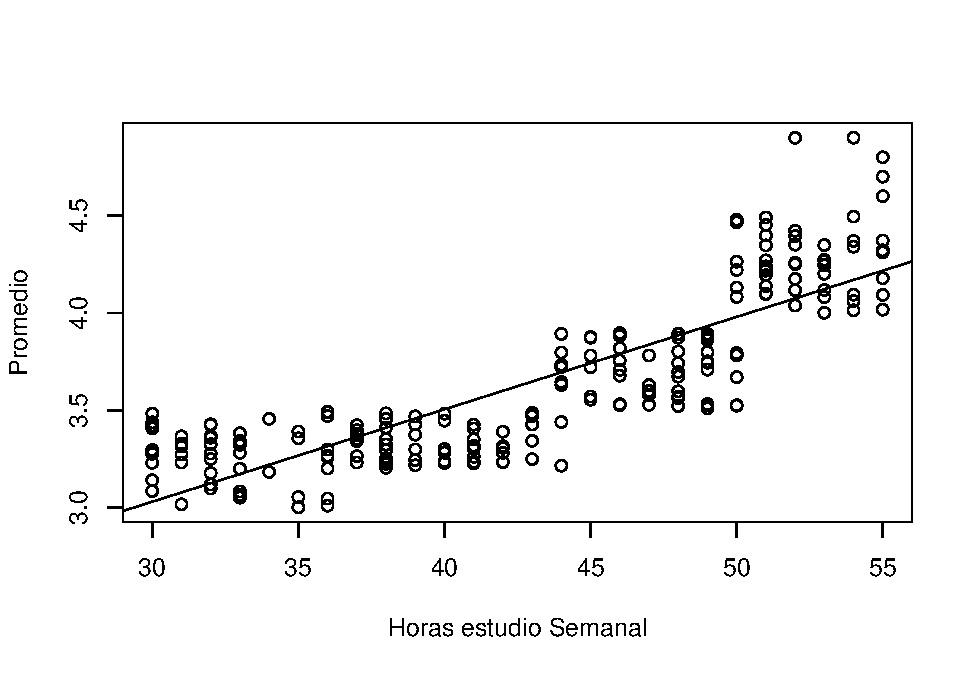
\includegraphics{Trabajo-Inferencia-estadística_files/figure-latex/unnamed-chunk-2-1.pdf}

\begin{verbatim}
## 
## Call:
## lm(formula = Base$`Promedio Primer Semestre` ~ Base$`Tiempo de estudio semanal (h)`, 
##     data = Base)
## 
## Residuals:
##      Min       1Q   Median       3Q      Max 
## -0.47946 -0.18797 -0.02077  0.16790  0.82512 
## 
## Coefficients:
##                                      Estimate Std. Error t value Pr(>|t|)    
## (Intercept)                           1.60647    0.09118   17.62   <2e-16 ***
## Base$`Tiempo de estudio semanal (h)`  0.04747    0.00208   22.82   <2e-16 ***
## ---
## Signif. codes:  0 '***' 0.001 '**' 0.01 '*' 0.05 '.' 0.1 ' ' 1
## 
## Residual standard error: 0.2344 on 218 degrees of freedom
## Multiple R-squared:  0.705,  Adjusted R-squared:  0.7036 
## F-statistic: 520.9 on 1 and 218 DF,  p-value: < 2.2e-16
\end{verbatim}

entonces el modelo estimado será
\[ (promedio)_i=1.60647+0.04747(Num.Horas)_i\] es decir por cada unidad
que cambia en el número de horas la nota promedio aumenta en 0.04747
unidades y cuando se da que no hay que no hay horas de estudio la nota
promedio estimada será de 1.6.

Es posbible observar la relación bien definida y ademas de causalidad
donde el modelo propuesto es capaz de explicar el 70.36\% de la variación
en la nota promedio.

\newpage

\hypertarget{regresiuxf3n-lineal-muxfaltiple}{%
\subsection{Regresión Lineal Múltiple}\label{regresiuxf3n-lineal-muxfaltiple}}

Observando las correlaciones entre las variables y las posibles
explicaciones unilaterales

procederemos a hacer la selccción del mejor modelo por el proceso de
Stepwise

\begin{verbatim}
## Start:  AIC=-621.01
## Base$`Promedio Primer Semestre` ~ Género + `Estrato social` + 
##     `Edad (Años)` + `PUNTAJE MATEMÁTICAS` + `PUNTAJE C. NATURALES` + 
##     `PUNTAJE INGLES` + `Tiempo de estudio semanal (h)` + `¿Realiza actividades extracurriculares?` + 
##     `¿Repasa los temas vistos en clase?` + `¿A cuántas tutorias asistió durante el semestre?`
## 
##                                                      Df Sum of Sq    RSS
## - `¿Realiza actividades extracurriculares?`           1    0.0034 11.518
## - Género                                              1    0.0049 11.519
## - `PUNTAJE C. NATURALES`                              1    0.0050 11.519
## - `¿A cuántas tutorias asistió durante el semestre?`  1    0.0069 11.521
## - `Estrato social`                                    1    0.0077 11.522
## - `PUNTAJE INGLES`                                    1    0.0090 11.523
## - `PUNTAJE MATEMÁTICAS`                               1    0.0151 11.529
## - `Edad (Años)`                                       1    0.0288 11.543
## - `¿Repasa los temas vistos en clase?`                4    0.3504 11.865
## <none>                                                            11.514
## - `Tiempo de estudio semanal (h)`                     1   27.5859 39.100
##                                                          AIC
## - `¿Realiza actividades extracurriculares?`          -622.95
## - Género                                             -622.92
## - `PUNTAJE C. NATURALES`                             -622.92
## - `¿A cuántas tutorias asistió durante el semestre?` -622.88
## - `Estrato social`                                   -622.86
## - `PUNTAJE INGLES`                                   -622.84
## - `PUNTAJE MATEMÁTICAS`                              -622.72
## - `Edad (Años)`                                      -622.46
## - `¿Repasa los temas vistos en clase?`               -622.42
## <none>                                               -621.01
## - `Tiempo de estudio semanal (h)`                    -354.05
## 
## Step:  AIC=-622.95
## Base$`Promedio Primer Semestre` ~ Género + `Estrato social` + 
##     `Edad (Años)` + `PUNTAJE MATEMÁTICAS` + `PUNTAJE C. NATURALES` + 
##     `PUNTAJE INGLES` + `Tiempo de estudio semanal (h)` + `¿Repasa los temas vistos en clase?` + 
##     `¿A cuántas tutorias asistió durante el semestre?`
## 
##                                                      Df Sum of Sq    RSS
## - Género                                              1    0.0048 11.522
## - `PUNTAJE C. NATURALES`                              1    0.0064 11.524
## - `¿A cuántas tutorias asistió durante el semestre?`  1    0.0064 11.524
## - `Estrato social`                                    1    0.0080 11.526
## - `PUNTAJE INGLES`                                    1    0.0092 11.527
## - `PUNTAJE MATEMÁTICAS`                               1    0.0166 11.534
## - `¿Repasa los temas vistos en clase?`                4    0.3481 11.866
## - `Edad (Años)`                                       1    0.0298 11.547
## <none>                                                            11.518
## - `Tiempo de estudio semanal (h)`                     1   27.5827 39.100
##                                                          AIC
## - Género                                             -624.85
## - `PUNTAJE C. NATURALES`                             -624.82
## - `¿A cuántas tutorias asistió durante el semestre?` -624.82
## - `Estrato social`                                   -624.79
## - `PUNTAJE INGLES`                                   -624.77
## - `PUNTAJE MATEMÁTICAS`                              -624.63
## - `¿Repasa los temas vistos en clase?`               -624.39
## - `Edad (Años)`                                      -624.38
## <none>                                               -622.95
## - `Tiempo de estudio semanal (h)`                    -356.05
## 
## Step:  AIC=-624.85
## Base$`Promedio Primer Semestre` ~ `Estrato social` + `Edad (Años)` + 
##     `PUNTAJE MATEMÁTICAS` + `PUNTAJE C. NATURALES` + `PUNTAJE INGLES` + 
##     `Tiempo de estudio semanal (h)` + `¿Repasa los temas vistos en clase?` + 
##     `¿A cuántas tutorias asistió durante el semestre?`
## 
##                                                      Df Sum of Sq    RSS
## - `¿A cuántas tutorias asistió durante el semestre?`  1    0.0057 11.528
## - `Estrato social`                                    1    0.0072 11.530
## - `PUNTAJE C. NATURALES`                              1    0.0074 11.530
## - `PUNTAJE INGLES`                                    1    0.0086 11.531
## - `PUNTAJE MATEMÁTICAS`                               1    0.0188 11.541
## - `¿Repasa los temas vistos en clase?`                4    0.3437 11.866
## - `Edad (Años)`                                       1    0.0318 11.554
## <none>                                                            11.522
## - `Tiempo de estudio semanal (h)`                     1   27.8812 39.404
##                                                          AIC
## - `¿A cuántas tutorias asistió durante el semestre?` -626.74
## - `Estrato social`                                   -626.72
## - `PUNTAJE C. NATURALES`                             -626.71
## - `PUNTAJE INGLES`                                   -626.69
## - `PUNTAJE MATEMÁTICAS`                              -626.50
## - `¿Repasa los temas vistos en clase?`               -626.39
## - `Edad (Años)`                                      -626.25
## <none>                                               -624.85
## - `Tiempo de estudio semanal (h)`                    -356.35
## 
## Step:  AIC=-626.74
## Base$`Promedio Primer Semestre` ~ `Estrato social` + `Edad (Años)` + 
##     `PUNTAJE MATEMÁTICAS` + `PUNTAJE C. NATURALES` + `PUNTAJE INGLES` + 
##     `Tiempo de estudio semanal (h)` + `¿Repasa los temas vistos en clase?`
## 
##                                        Df Sum of Sq    RSS     AIC
## - `PUNTAJE C. NATURALES`                1    0.0068 11.535 -628.62
## - `Estrato social`                      1    0.0068 11.535 -628.61
## - `PUNTAJE INGLES`                      1    0.0096 11.538 -628.56
## - `PUNTAJE MATEMÁTICAS`                 1    0.0235 11.552 -628.30
## - `Edad (Años)`                         1    0.0306 11.559 -628.16
## - `¿Repasa los temas vistos en clase?`  4    0.3607 11.889 -627.97
## <none>                                              11.528 -626.74
## - `Tiempo de estudio semanal (h)`       1   28.0017 39.530 -357.65
## 
## Step:  AIC=-628.62
## Base$`Promedio Primer Semestre` ~ `Estrato social` + `Edad (Años)` + 
##     `PUNTAJE MATEMÁTICAS` + `PUNTAJE INGLES` + `Tiempo de estudio semanal (h)` + 
##     `¿Repasa los temas vistos en clase?`
## 
##                                        Df Sum of Sq    RSS     AIC
## - `Estrato social`                      1    0.0074 11.542 -630.47
## - `PUNTAJE INGLES`                      1    0.0113 11.546 -630.40
## - `PUNTAJE MATEMÁTICAS`                 1    0.0220 11.557 -630.20
## - `Edad (Años)`                         1    0.0297 11.565 -630.05
## - `¿Repasa los temas vistos en clase?`  4    0.3580 11.893 -629.89
## <none>                                              11.535 -628.62
## - `Tiempo de estudio semanal (h)`       1   28.0882 39.623 -359.13
## 
## Step:  AIC=-630.47
## Base$`Promedio Primer Semestre` ~ `Edad (Años)` + `PUNTAJE MATEMÁTICAS` + 
##     `PUNTAJE INGLES` + `Tiempo de estudio semanal (h)` + `¿Repasa los temas vistos en clase?`
## 
##                                        Df Sum of Sq    RSS     AIC
## - `PUNTAJE INGLES`                      1    0.0117 11.554 -632.25
## - `PUNTAJE MATEMÁTICAS`                 1    0.0221 11.564 -632.05
## - `Edad (Años)`                         1    0.0288 11.571 -631.93
## - `¿Repasa los temas vistos en clase?`  4    0.3524 11.895 -631.86
## <none>                                              11.542 -630.47
## - `Tiempo de estudio semanal (h)`       1   28.1032 39.646 -361.00
## 
## Step:  AIC=-632.25
## Base$`Promedio Primer Semestre` ~ `Edad (Años)` + `PUNTAJE MATEMÁTICAS` + 
##     `Tiempo de estudio semanal (h)` + `¿Repasa los temas vistos en clase?`
## 
##                                        Df Sum of Sq    RSS     AIC
## - `PUNTAJE MATEMÁTICAS`                 1    0.0224 11.577 -633.82
## - `¿Repasa los temas vistos en clase?`  4    0.3441 11.898 -633.79
## - `Edad (Años)`                         1    0.0338 11.588 -633.61
## <none>                                              11.554 -632.25
## - `Tiempo de estudio semanal (h)`       1   28.3563 39.910 -361.54
## 
## Step:  AIC=-633.82
## Base$`Promedio Primer Semestre` ~ `Edad (Años)` + `Tiempo de estudio semanal (h)` + 
##     `¿Repasa los temas vistos en clase?`
## 
##                                        Df Sum of Sq    RSS     AIC
## - `¿Repasa los temas vistos en clase?`  4    0.3454 11.922 -635.35
## - `Edad (Años)`                         1    0.0290 11.606 -635.27
## <none>                                              11.577 -633.82
## - `Tiempo de estudio semanal (h)`       1   28.6916 40.268 -361.58
## 
## Step:  AIC=-635.35
## Base$`Promedio Primer Semestre` ~ `Edad (Años)` + `Tiempo de estudio semanal (h)`
## 
##                                   Df Sum of Sq    RSS     AIC
## - `Edad (Años)`                    1    0.0583 11.980 -636.28
## <none>                                         11.922 -635.35
## - `Tiempo de estudio semanal (h)`  1   28.4776 40.400 -368.86
## 
## Step:  AIC=-636.28
## Base$`Promedio Primer Semestre` ~ `Tiempo de estudio semanal (h)`
## 
##                                   Df Sum of Sq    RSS     AIC
## <none>                                         11.980 -636.28
## - `Tiempo de estudio semanal (h)`  1    28.627 40.607 -369.73
\end{verbatim}

\begin{verbatim}
## 
## Call:
## lm(formula = Base$`Promedio Primer Semestre` ~ `Tiempo de estudio semanal (h)`, 
##     data = Base)
## 
## Coefficients:
##                     (Intercept)  `Tiempo de estudio semanal (h)`  
##                         1.60647                          0.04747
\end{verbatim}

Es posible observar que el mejor modelo que se puede tener es el modelo lineal planteado anteriormente.

\newpage

\hypertarget{anova-anuxe1lisis-de-la-varianza}{%
\section{ANOVA (Análisis de la varianza)}\label{anova-anuxe1lisis-de-la-varianza}}

Primero observemos como se comporta la relación entre el promedio del
primer semestre y el estrato social

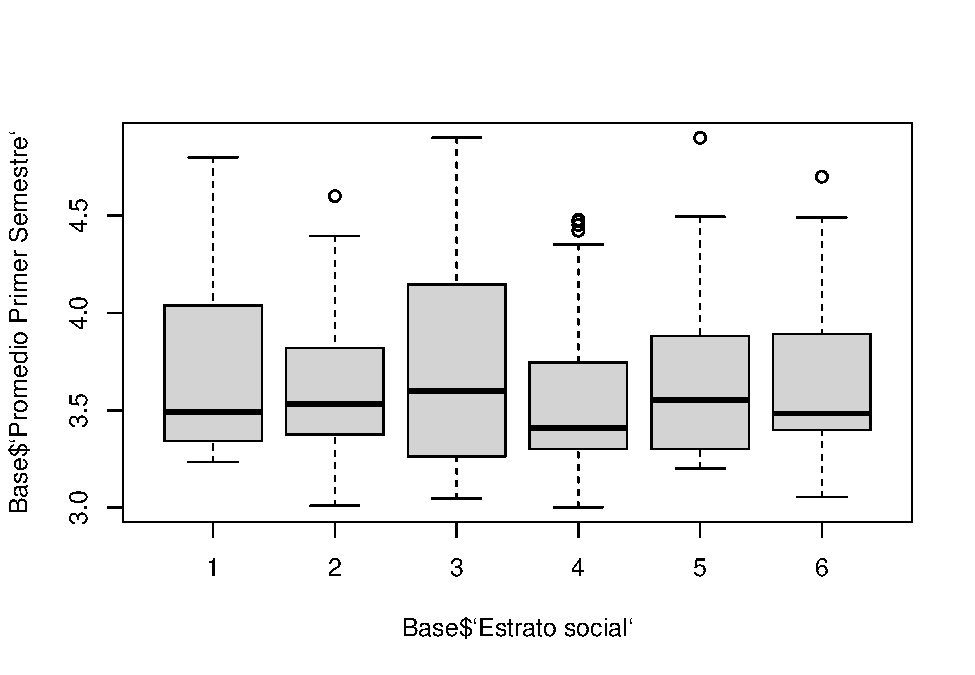
\includegraphics{Trabajo-Inferencia-estadística_files/figure-latex/unnamed-chunk-4-1.pdf}

\begin{verbatim}
## Call:
##    aov(formula = regreAnova)
## 
## Terms:
##                 Base$`Estrato social` Residuals
## Sum of Squares                0.02106  40.58594
## Deg. of Freedom                     1       218
## 
## Residual standard error: 0.4314789
## Estimated effects may be unbalanced
\end{verbatim}

podemos ver que se NO se rechaza la hipotésis nula de la igualdad de medias , por lo tanto
el estrato social no influye en el promedio de manera significativa.

\hypertarget{conclusiones}{%
\section{Conclusiones}\label{conclusiones}}

Es posible concluir que las notas de las pruebas icfes no son útiles para precedir el promedio de
los estudiantes que entran a a facultad de psicologia , sin embargo en la busqueda a la respuesta de este interrogante encontramos una relación entre el número de horas dedicacas al estudio y el incremento dela nota promedio de los estudiantes . Además , se encontró un modelo para poder precedicir con una acertividad del 70\% aproximadamente.

\hypertarget{references}{%
\section{References}\label{references}}

\begingroup
\setlength{\parindent}{-0.5in}
\setlength{\leftskip}{0.5in}

Hernández, F. (2021, 26 julio). Manual de R. R manual.
\url{https://fhernanb.github.io/Manual-de-R/}

Sancho, R. S. (2020). filter() \textbar{} Programación en R. R.
\url{https://rsanchezs.gitbooks.io/rprogramming/content/chapter9/filter.html}

RPubs - Contrastes de hipÃ3tesis en R. (2018, 25 abril). Hipotesis.
\url{https://rpubs.com/Jo_/contrastes_hipotesis_ttest}

RPubs - Analisis\_Univariable. (2014, 27 octubre). Analisis.
\url{https://rpubs.com/dsulmont/37910}

RPubs - 3.3.2. Tablas de frecuencias agrupadas en R. (2021, 29 junio).
tablas. \url{https://rpubs.com/hllinas/R_Tablas_agrupadas}

27 R Markdown \textbar{} \_main.utf8. (2020). Rmarkdown.
\url{https://es.r4ds.hadley.nz/r-markdown.html}

Zhu, H. (2021, 19 febrero). Create Awesome HTML Table with knitr::kable
and kableExtra. tabla.
\url{https://cran.r-project.org/web/packages/kableExtra/vignettes/awesome_table_in_html.html\#Position}

\hypertarget{refs}{}
\begin{CSLReferences}{0}{0}
\end{CSLReferences}

\endgroup


\end{document}
